\section{Mechanisms}

As mentioned earlier, we implemented two backside touch input based
mechanisms and a standard soft-QWERTY keyboard. The details of each
are as following:

\subsection{QWERTY}

This was a standard soft QWERTY keyboard [Figure], with no special
modifications. The keyboard supported multitouch, which means the
users could select the next character to be entered without releasing
the currently selected one. The keys turned blue on click, so that the
user gets appropriate feedback. The top quarter of the screen was a
scrollable textfield, which displayed the text that was being entered.

\subsection{Backside QWERTY}
\subsubsection{Description}

This mechanism used the standard QWERTY layout, but with a few
modifications. In this mechanism, the user could place his fingers on
the backside screen and it would result in a cursor on the front
screen at a location that is vertically above the touch point. This
way users could move around multiple cursors at the same time, using
multiple fingers. To input a particular character, the user was
required to go select a particular key with the cursor and then touch
the front screen anywhere to signal input. Figure 3 shows a user trying to reach out for some characters on the backside-QWERTY mechanism.

\begin{figure}
    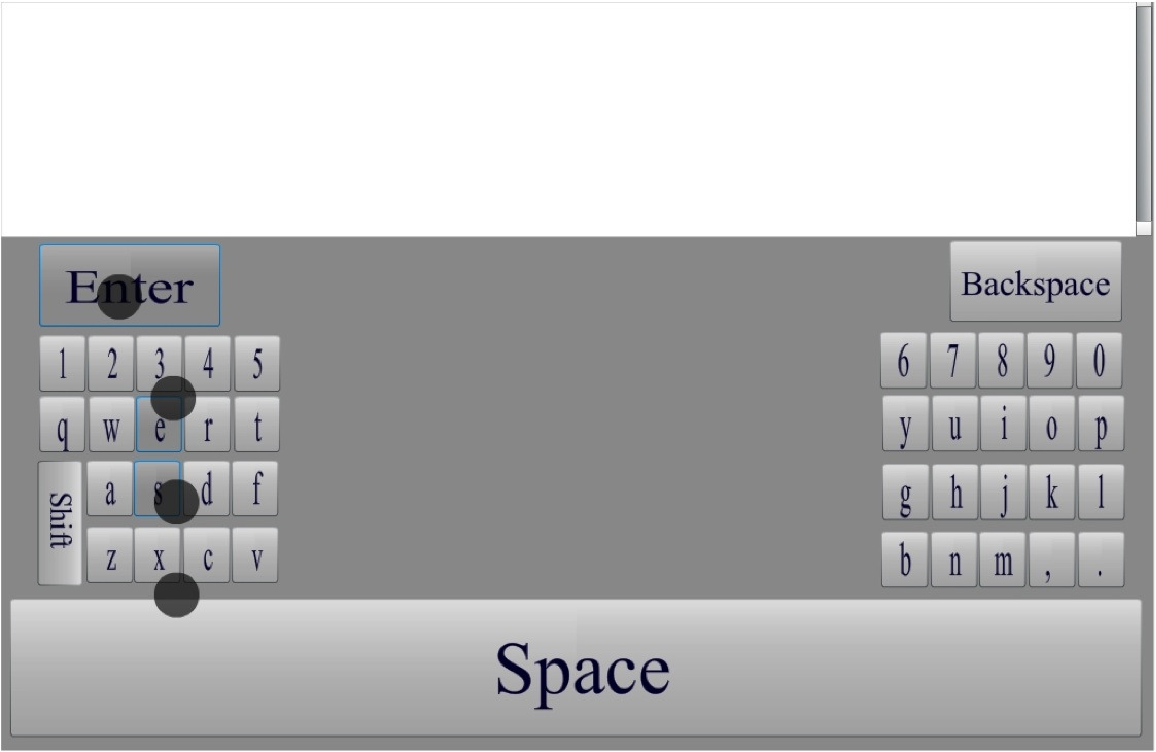
\includegraphics[scale=0.45]{Figures/backside.pdf} 
    \caption{Screenshot of backside-QWERTY with user's fingers on the
      backside screen}
\end{figure}

\subsubsection{Design evolution}

The interface went through two iterations before getting its final
shape. The first version used pressure as a method to signal
input. However, usability tests suggested that being able to control
the amount of pressure being applied is hard for users. Since the
users were already applying some pressure to drag the cursors around,
it turned out to be confusing for them.

Therefore, the second version of the interface used cursor destroy
events as a method to signal text input. In simple words, the
interface would accept a character as input if the corresponding key
had a cursor destroy event over it. However, in this case the
usability tests suggested that choosing not to give an input would
mean that the user needs to go to section of the screen that has no
keys and then choose to remove the touch/cursor. Also, the chances of
giving accidental inputs, by accidental destroy events increased
menifold. Both these factors resulted in additional overhead in terms
of time.

As a result we finally shifted to touching the front panel once the
character has been selected, as the method to signal input.

In the first version we had also modified the keyboard layout to match
the finger to key mappings on a QWERTY keyboard. However,
after the usability test, we realized that users were still doing
visual search for keys instead of using their pre-existing knowledge
of QWERTY. Therefore, a QWERTY layout in this case turned out to be
more predictable and usable.Moreover, the size of the Space, Backspace
and Enter keys was increased so that they are easy to select.

\subsection{Chording mechanism}
\subsubsection{Description}

\begin{figure*}
    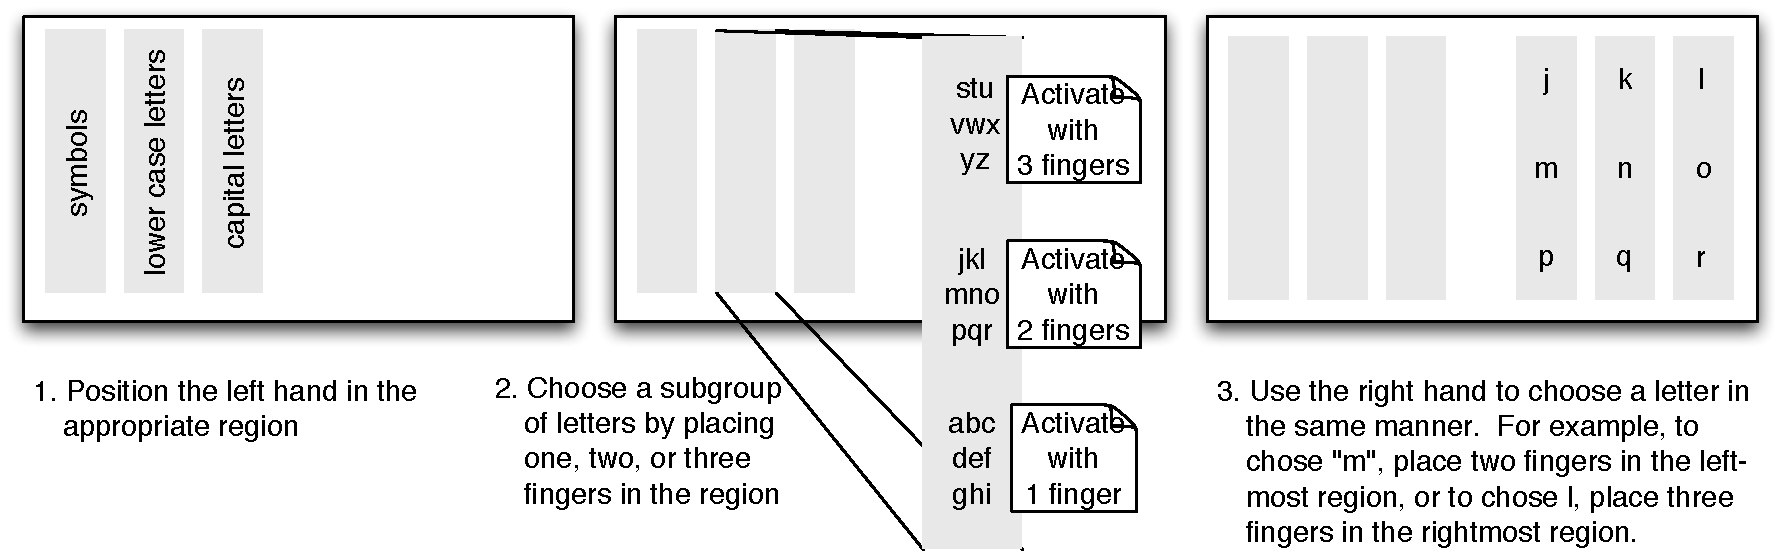
\includegraphics[width=\textwidth]{Figures/chording_explaination.pdf} 
    \caption{Enter the character ``l'' using the chording mechansims.
      Note that all three steps can be performed simultaneously, for
      proficient users.}
    \label{fig:chording_explaination}
\end{figure*} 

The lack of tactile feedback has often been cited as the primary
problem with touchscreen-based keyboards.  Tactile feedback allows a
user to move their hands around the keyboard without looking, and to
therefore focus on the text they are typing.  The chording mechanism
was designed to allow the user to exploit their proprioception (the
sense of the relative postions of one's body) rather than tactile
feedback, in order to form and exploit kinesthetic memory
(short-feedback memory in the nervous system that bypasses cognative
processing for repetative tasks, often called ``muscle-memory'').
Since gross motor movements provide better proprioception, the
mechanism was designed to reduce requirements for precise movement.

The chording mechanism only requires that the user extend and contract
their fingers (e.g. move their fingers in the horizontal axis in the
natural pose).  There are three regions for each hand, determined
exclusively by the distance from the edge of the screen.  In the left
hand, each region corresponds to a character class: upper-case,
lower-case or symbols.  Within these classes, the number of fingers
touching the region determines one of three subgroups in the class,
with nine characters in each subgroup.  The nine characters are broken
up into three groups, and an individual character is selected using
the same mechanism on the right hand
(Figure~\ref{fig:chording_explaination}).

In our implementation, the number of fingers activating a region is
indicated by color changes to the activated regions, in addition to
the translucent circles representing the location of the fingers.
The user can use these circles to position their fingers in the correct
locations.  They then touche anywhere on the front screen to
indicate a character input.  When the user is learning how to use the
chording mechanism, they can enter a character using the step-by-step
process described above.  As they become more familiar, however, then
can enter chords by touching the device with both hands, in the
correct location, simultaneously
.
Similar to backside QWERTY and QWERTY, the top quarter of the screen
was a scrollable textfield, which displayed the text that was being
entered.

\begin{figure}
    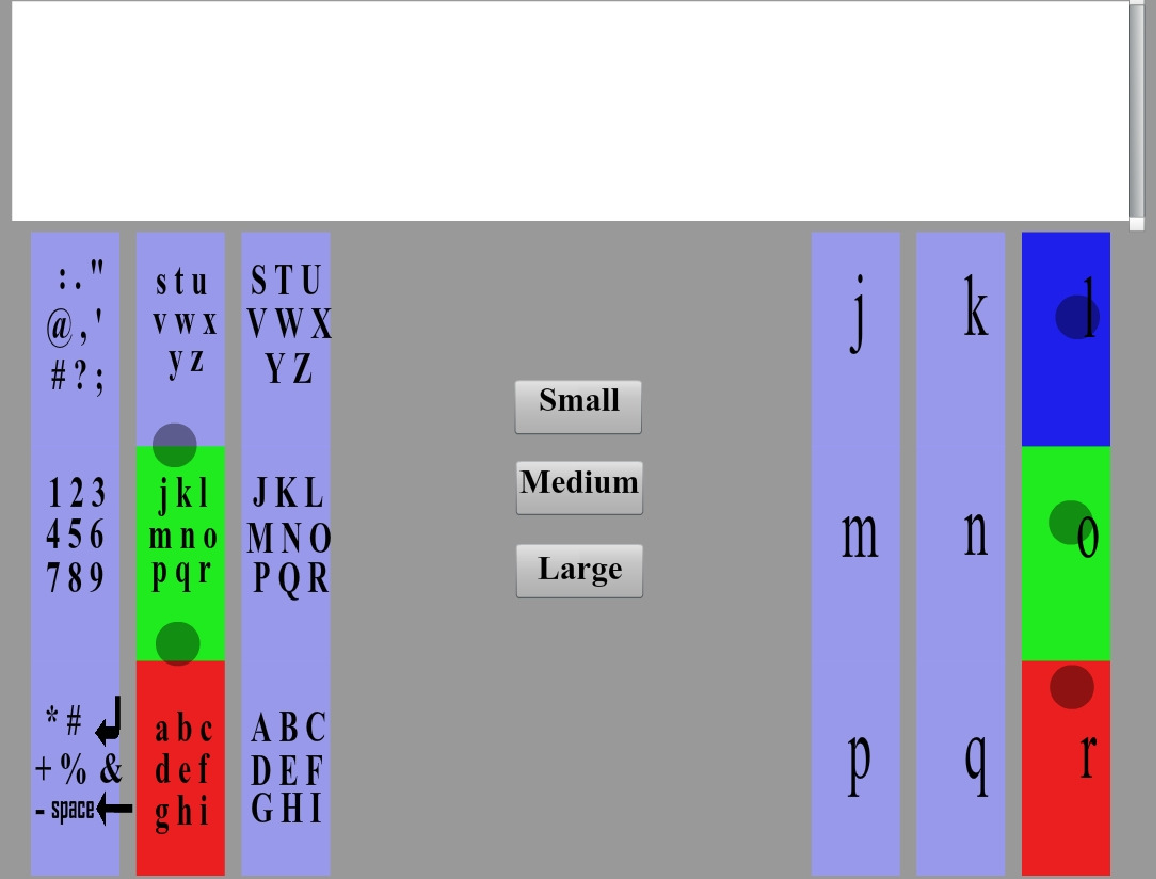
\includegraphics[scale=0.45]{Figures/chording.pdf} 
    \caption{Screenshot of chording mechanism with user's fingers on
      the backside screen trying to form a chord}
\end{figure} 
\subsubsection{Design Evolution}

As in the case of backside QWERTY, after the first round of usability
testing, it was observed that users find it hard to control the
pressure being applied by the fingers. Therefore, in the final version
of the mechanism the users could touch the front screen to signal text
input for the character selected by the chords.

Usability testing suggested that the finger sizes and areas in which
users can move comfortably vary a lot. Therefore, in the final version
the users were allowed to select from large/medium/small setting
[Figure], that determined the width of the zones. Users, who had
smaller reach, could use these settings to optimize the area of
movement.
